\documentclass[a4paper]{article}
\usepackage{xcolor}
\usepackage{graphicx} % Required for inserting images
\pagecolor{black}
\color{white}
\usepackage{listings}

\title{EE 236 Devices Lab \\ Lab - 03}
\author{Anupam Rawat, 22b3982}
\date{${24^{th}}$ August, 2024}

\begin{document}

\maketitle
\begin{center}
    \section*{Temperature and material dependence of PN diode, IV characteristics}    
\end{center}


\section{Dark I-V Characteristics of Photodiode}

\subsection{Aim of the experiment}
Obtain the dark I-V characteristics of the given photodiode for forward as
well as reverse bias

\subsection{Design}
\begin{figure}[h!]
    \centering
    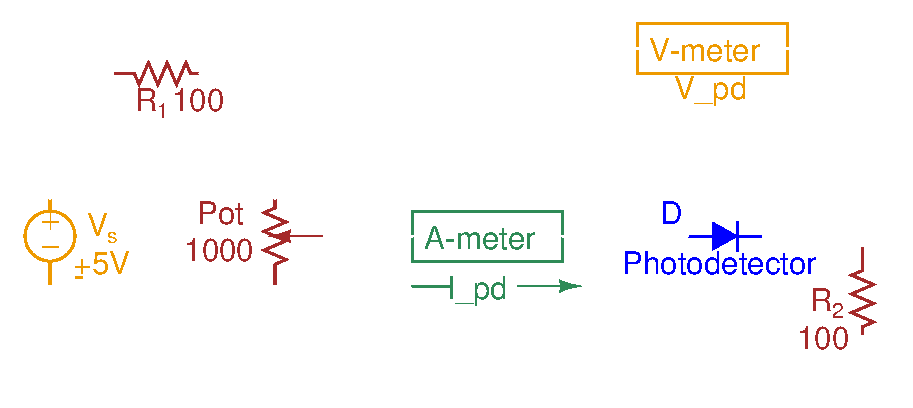
\includegraphics{Lab_3_Circuit_Design_Exp_1.eps}
    \caption{Caption}
    \label{fig:enter-label}
\end{figure}

\newpage
\subsection{Forward Bias}
\begin{table}[h!]
\centering
\begin{tabular}{|c|c|c|c|c|c|}
\hline
\textbf{Vpd} & \textbf{Ipd} & \textbf{log(abs(I\_pd))} & \textbf{Vpd} & \textbf{Ipd} & \textbf{log(abs(I\_pd))} \\ \hline
0.50 & 1.00E-12 & -12 & 0.75 & 6.6  & 0.8195 \\ \hline
0.51 & 0.1      & -1  & 0.76 & 7    & 0.8451 \\ \hline
0.53 & 0.1      & -1  & 0.77 & 8.2  & 0.9138 \\ \hline
0.55 & 0.3      & -0.5229 & 0.78 & 8.6  & 0.9345 \\ \hline
0.56 & 0.4      & -0.3979 & 0.79 & 9.9  & 0.9956 \\ \hline
0.59 & 0.8      & -0.0969 & 0.80 & 11   & 1.0414 \\ \hline
0.60 & 1        & 0      & 0.81 & 11.8 & 1.0719 \\ \hline
0.62 & 1.4      & 0.1461 & 0.82 & 12.9 & 1.1106 \\ \hline
0.64 & 1.9      & 0.2788 & 0.83 & 13.9 & 1.1430 \\ \hline
0.65 & 2.2      & 0.3424 & 0.835 & 14.1 & 1.1492 \\ \hline
0.66 & 2.7      & 0.4314 & 0.84 & 16.2 & 1.2095 \\ \hline
0.67 & 3.2      & 0.5051 & 0.85 & 17.77 & 1.2497 \\ \hline
0.69 & 3.6      & 0.5563 & 0.86 & 19.4 & 1.2878 \\ \hline
0.70 & 4        & 0.6021 & 0.87 & 21.4 & 1.3304 \\ \hline
0.71 & 4.5      & 0.6532 & 0.88 & 22   & 1.3424 \\ \hline
0.72 & 5        & 0.6990 &       &      &        \\ \hline
0.73 & 5.6      & 0.7482 &       &      &        \\ \hline
0.74 & 5.8      & 0.7634 &       &      &        \\ \hline
\end{tabular}
\caption{$V_{pd}$ v/s $I_{pd}$}
\end{table}

\begin{table}[h!]
\centering
\begin{tabular}{|c|c|}
\hline
\textbf{Parameter} & \textbf{Value} \\ \hline
\textbf{slope}     & 12.1790547     \\ \hline
\textbf{intercept} & -7.2826286     \\ \hline
\textbf{$\eta$}       & 3.1580069      \\ \hline
\end{tabular}
\caption{Slope, Intercept and Ideality Factor for Forward Bias}
\label{tab:params}
\end{table}


\begin{figure}[h!]
    \centering
    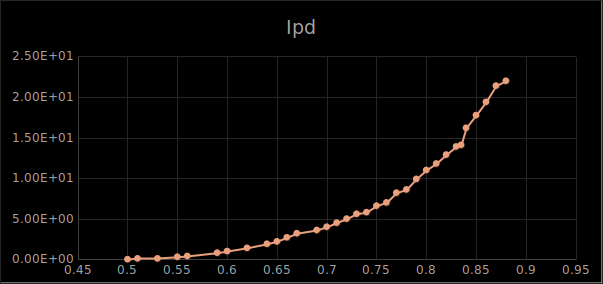
\includegraphics[width=1\linewidth]{Lab_3/inverted_Exp_1_Forward_Bias_V_I.png}
    \caption{I/V Characteristic Linear Scale}
\end{figure}

\newpage

\begin{figure}[h!]
    \centering
    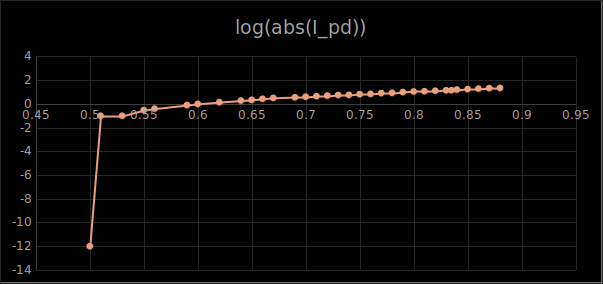
\includegraphics[width=1\linewidth]{Lab_3/inverted_Exp_1_Forward_Bias_log_V_I.png}
    \caption{I/V Characteristic Log Scale}
\end{figure}

\subsection{Reverse Bias}
\begin{table}[h!]
\centering
\begin{tabular}{|c|c|c|}
\hline
\textbf{Vd (mV)} & \textbf{Id (µA)} & \textbf{ln(abs(Id))} \\ \hline
-0.48 & -0.3 & -1.204 \\ \hline
-0.94 & -0.4 & -0.916 \\ \hline
-2.13 & -0.5 & -0.693 \\ \hline
-2.7 & -0.6 & -0.511 \\ \hline
-3.9 & -0.7 & -0.357 \\ \hline
-4.58 & -0.8 & -0.223 \\ \hline
\end{tabular}
\caption{Measurements of Vd, Id, and ln(abs(Id))}
\label{tab:voltage_current_log}
\end{table}


\begin{figure}[h!]
    \centering
    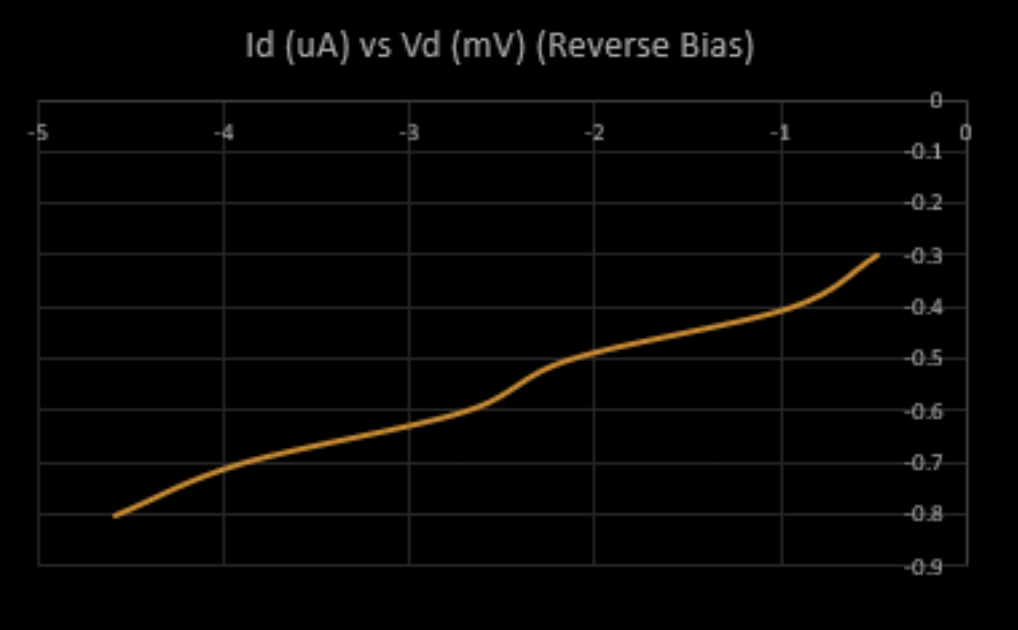
\includegraphics[width=0.7\linewidth]{inverted_re.png}
\end{figure}

\newpage
























\newpage

\section{Photodiode response to lights of different intensities and wavelengths}

\subsection{Aim of the Experiment}
Investigate the response of a photodiode to different intensities and wavelengths of light emitted by various LEDs and calculate the efficiency of each LED.

\subsection{Design}
\begin{figure}[h!]
    \centering
    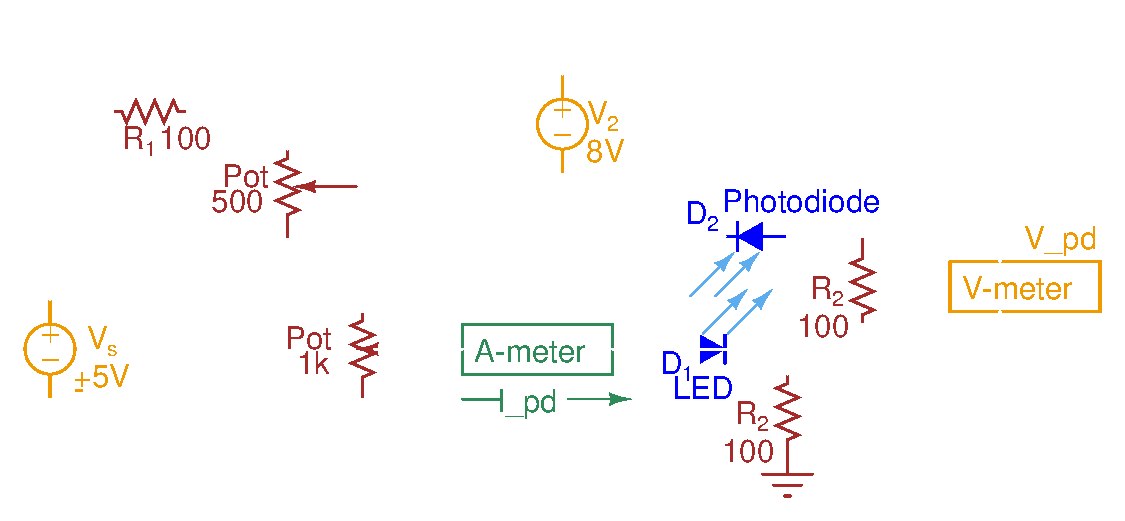
\includegraphics[scale=0.8]{Lab_3_Circuit_Design_Exp_2.eps}
    \caption{Caption}
    \label{fig:enter-label}
\end{figure}

\subsection{$V_{out}$ and $I_{out}$ of LEDs at different intensities}

\begin{table}[h!]
\centering
\begin{tabular}{|c|c|c|c|c|c|}
\hline
\multicolumn{3}{|c|}{\textbf{Red LED (750 nm)}} & \multicolumn{3}{c|}{\textbf{Blue LED (450 nm)}} \\ \hline
\textbf{I\_out (mA)} & \textbf{V\_out (mv)} & \textbf{Intensity} & \textbf{I\_out (mA)} & \textbf{V\_out (mV)} & \textbf{Intensity} \\ \hline
2 & 0.24 & 1000 & 0.301 & 13.9 & 1000 \\ \hline
3 & 0.32 & 1500 & 0.416 & 19.3 & 1500 \\ \hline
4 & 0.38 & 2000 & 0.572 & 28.1 & 2000 \\ \hline
\multicolumn{3}{|c|}{\textbf{Green LED (520 nm)}} & \multicolumn{3}{c|}{\textbf{IR LED (950 nm)}} \\ \hline
\textbf{I\_out} & \textbf{V\_out (mV)} & \textbf{Intensity} & \textbf{I\_out} & \textbf{V\_out} & \textbf{Intensity} \\ \hline
0.188 & 33.2 & 1000 & 4.51 & 0.303 & 1000 \\ \hline
0.294 & 52.4 & 1500 & 5.17 & 0.359 & 1500 \\ \hline
0.371 & 66.6 & 2000 & 6.28 & 0.456 & 2000 \\ \hline
\end{tabular}
\caption{Photodiode response to different LEDs at various intensities}
\label{tab:led_response}
\end{table}

\newpage
\begin{table}[h!]
\centering
\begin{tabular}{|c|c|c|c|}
\hline
\multicolumn{2}{|c|}{\textbf{Red LED (750 nm)}} & \multicolumn{2}{c|}{\textbf{IR LED (950 nm)}} \\ \hline
\textbf{Intensity} & \textbf{Efficiency} & \textbf{Intensity} & \textbf{Efficiency} \\ \hline
1000 & 12 & 1000 & 6.72 \\ \hline
1500 & 10.67 & 1500 & 6.94 \\ \hline
2000 & 9.5 & 2000 & 7.26 \\ \hline
\end{tabular}
\caption{Response of Red and IR LEDs at various intensities}
\label{tab:red_ir_led}
\end{table}

\vspace{1em}

\begin{table}[h!]
\centering
\begin{tabular}{|c|c|c|c|}
\hline
\multicolumn{2}{|c|}{\textbf{Green LED (520 nm)}} & \multicolumn{2}{c|}{\textbf{Blue LED (450 nm)}} \\ \hline
\textbf{Intensity} & \textbf{Efficiency} & \textbf{Intensity} & \textbf{Efficiency} \\ \hline
1000 & 17.66 & 1000 & 4.62 \\ \hline
1500 & 17.82 & 1500 & 4.64 \\ \hline
2000 & 17.95 & 2000 & 4.91 \\ \hline
\end{tabular}
\caption{Response of Green and Blue LEDs at various intensities}
\label{tab:green_blue_led}
\end{table}

\begin{figure}[h!]
    \centering
    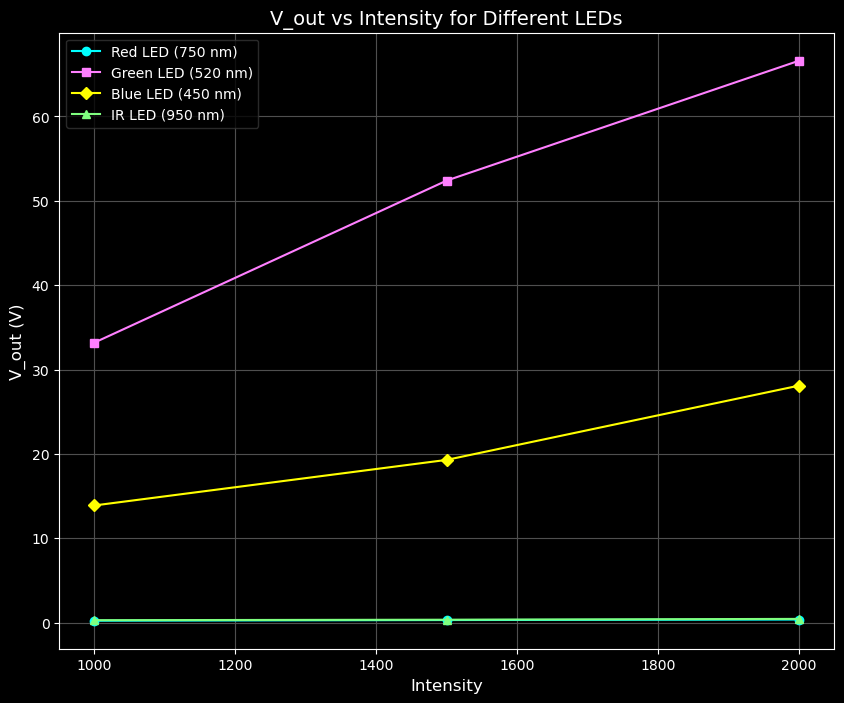
\includegraphics[width=1\linewidth]{Lab_3/inverted_Exp_2_V_out_vs_Intensity.png}
    \caption{$V_{out}$ v/s Intensity for each LED}
    \label{fig:enter-label}
\end{figure}

\newpage

\begin{figure}[h!]
    \centering
    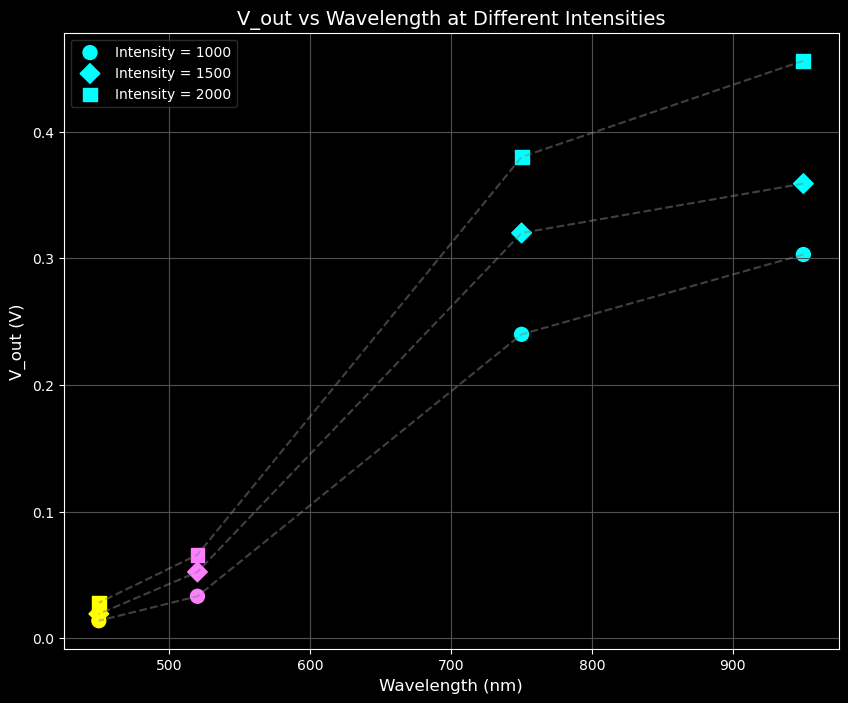
\includegraphics[width=1\linewidth]{Lab_3/inverted_Exp_2_V_out_vs_Wavelength.png}
    \caption{$V_{out}$ v/s Wavelength for each intensity}
    \label{fig:enter-label}
\end{figure}


\newpage




















\newpage
\section{Application of photodiode as optical signal sensor}
\subsection{Circuit Design}
\begin{figure}[ht]
    \centering
    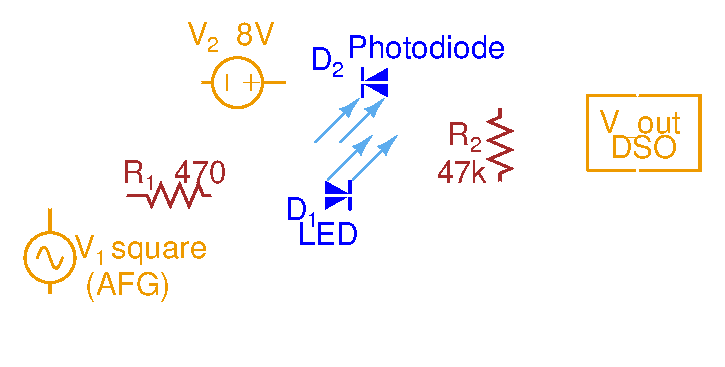
\includegraphics{Lab_3_Circuit_Design_Exp_3.eps}
    \caption{Experiment 3}
\end{figure}
\subsection{Rise time and Fall time for different Frequencies}

\begin{table}[h!]
\centering
\begin{tabular}{|c|c|c|}
\hline
\textbf{Frequency (kHz)} & \textbf{Rise Time (µs)} & \textbf{Fall Time (µs)} \\ \hline
1 & 5.070 & 3.957 \\ \hline
5 & 3.985 & 2.404 \\ \hline
10 & 3.393 & 2.021 \\ \hline
15 & 2.631 & 1.540 \\ \hline
20 & 2.411 & 1.321 \\ \hline
25 & 2.938 & 1.707 \\ \hline
30 & 2.307 & 2.141 \\ \hline
35 & 2.442 & 1.427 \\ \hline
\end{tabular}
\caption{Rise and Fall Times at Various Frequencies}
\label{tab:rise_fall_times}
\end{table}


\begin{figure}[h!]
    \centering
    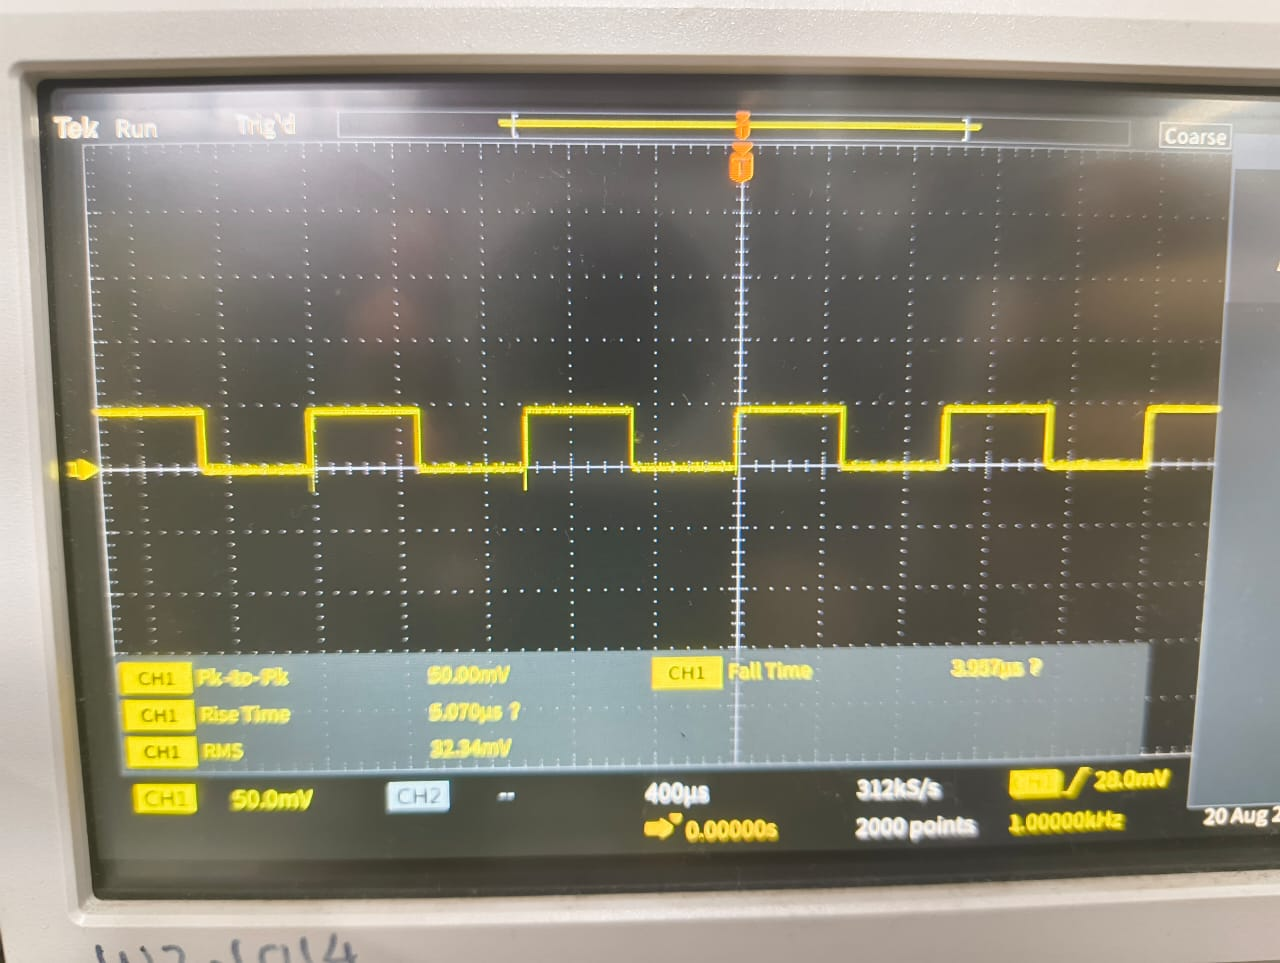
\includegraphics[width=0.8\linewidth]{1k.jpeg}
    \caption{For 1KHz}
\end{figure}

\begin{figure}[h!]
    \centering
    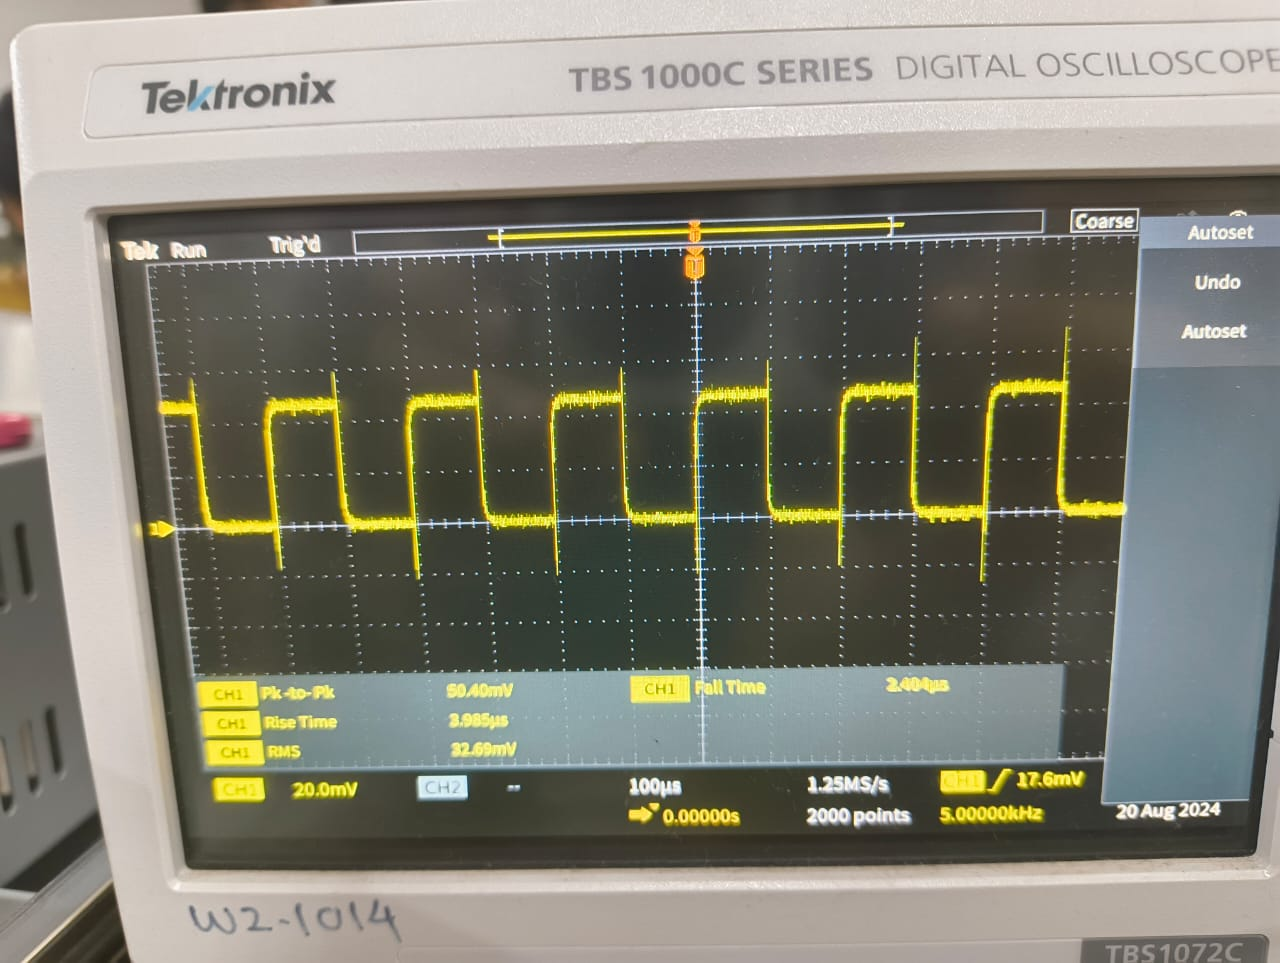
\includegraphics[width=0.8\linewidth]{5k.jpeg}
    \caption{For 5KHz}
\end{figure}

\begin{figure}[h!]
    \centering
    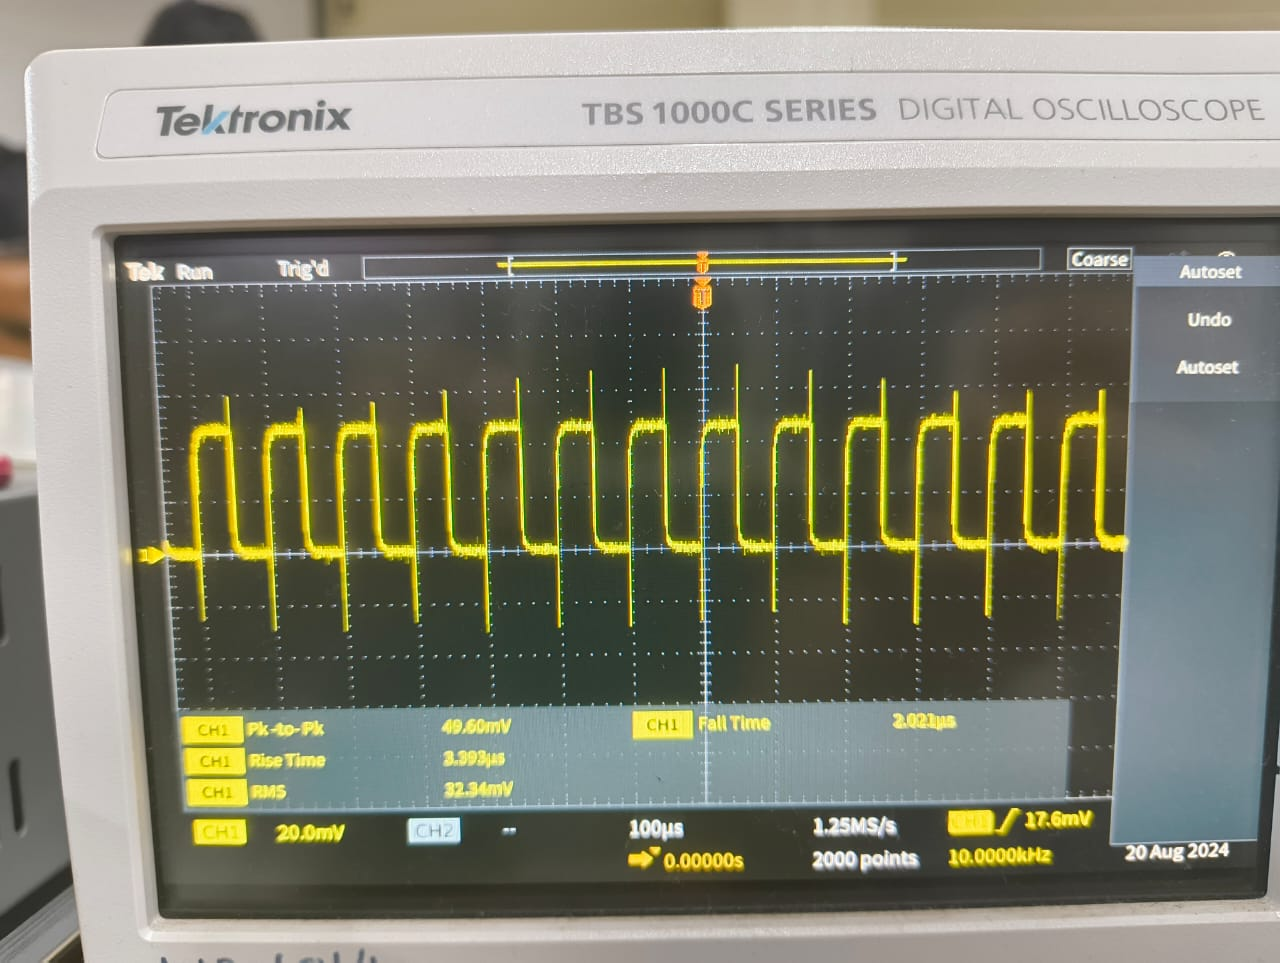
\includegraphics[width=0.8\linewidth]{10k.jpeg}
    \caption{For 10KHz}
\end{figure}

\begin{figure}[h!]
    \centering
    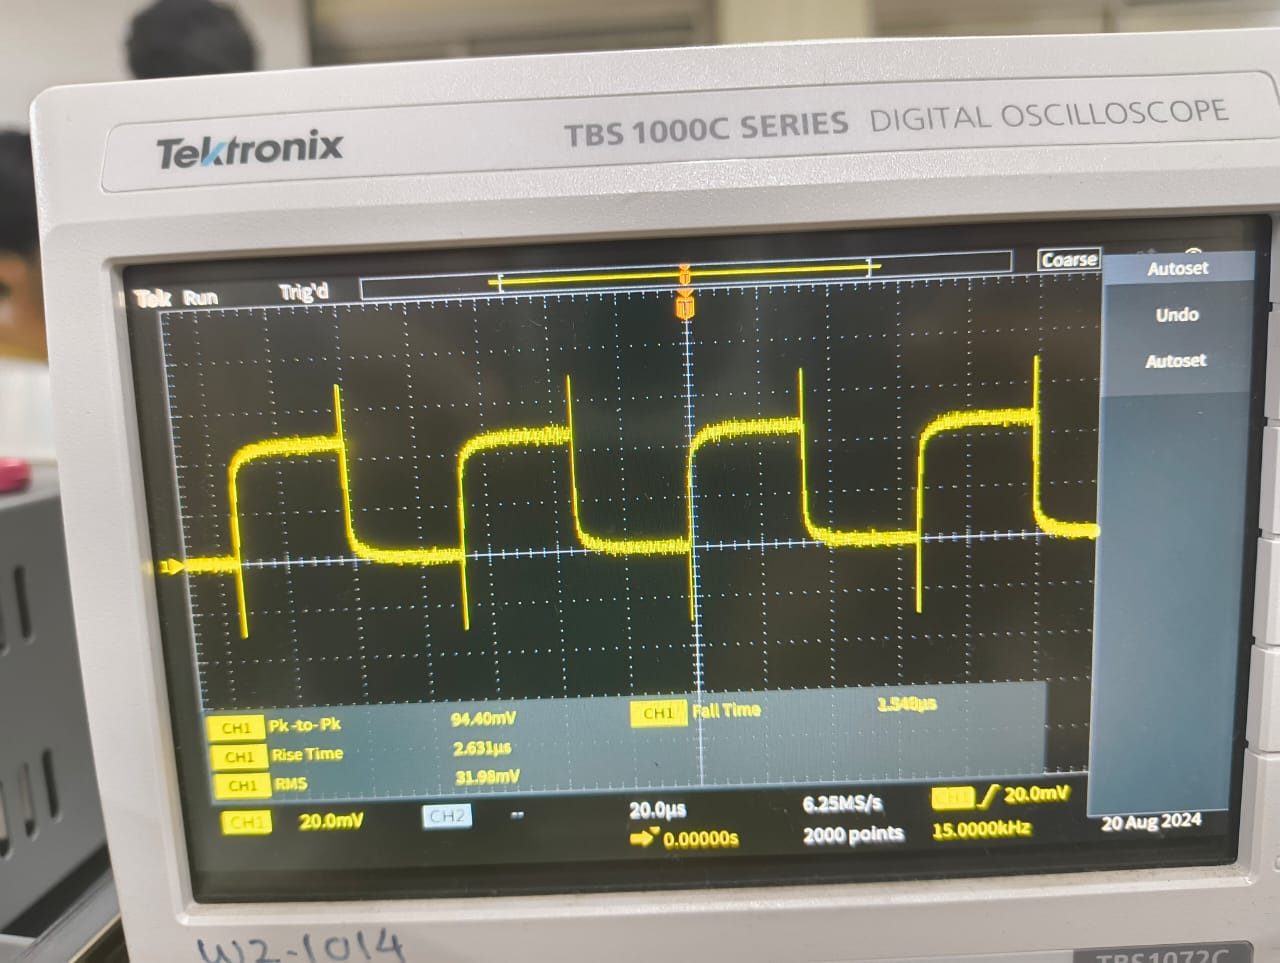
\includegraphics[width=0.8\linewidth]{15k.jpeg}
    \caption{For 15KHz}
\end{figure}

\begin{figure}[h!]
    \centering
    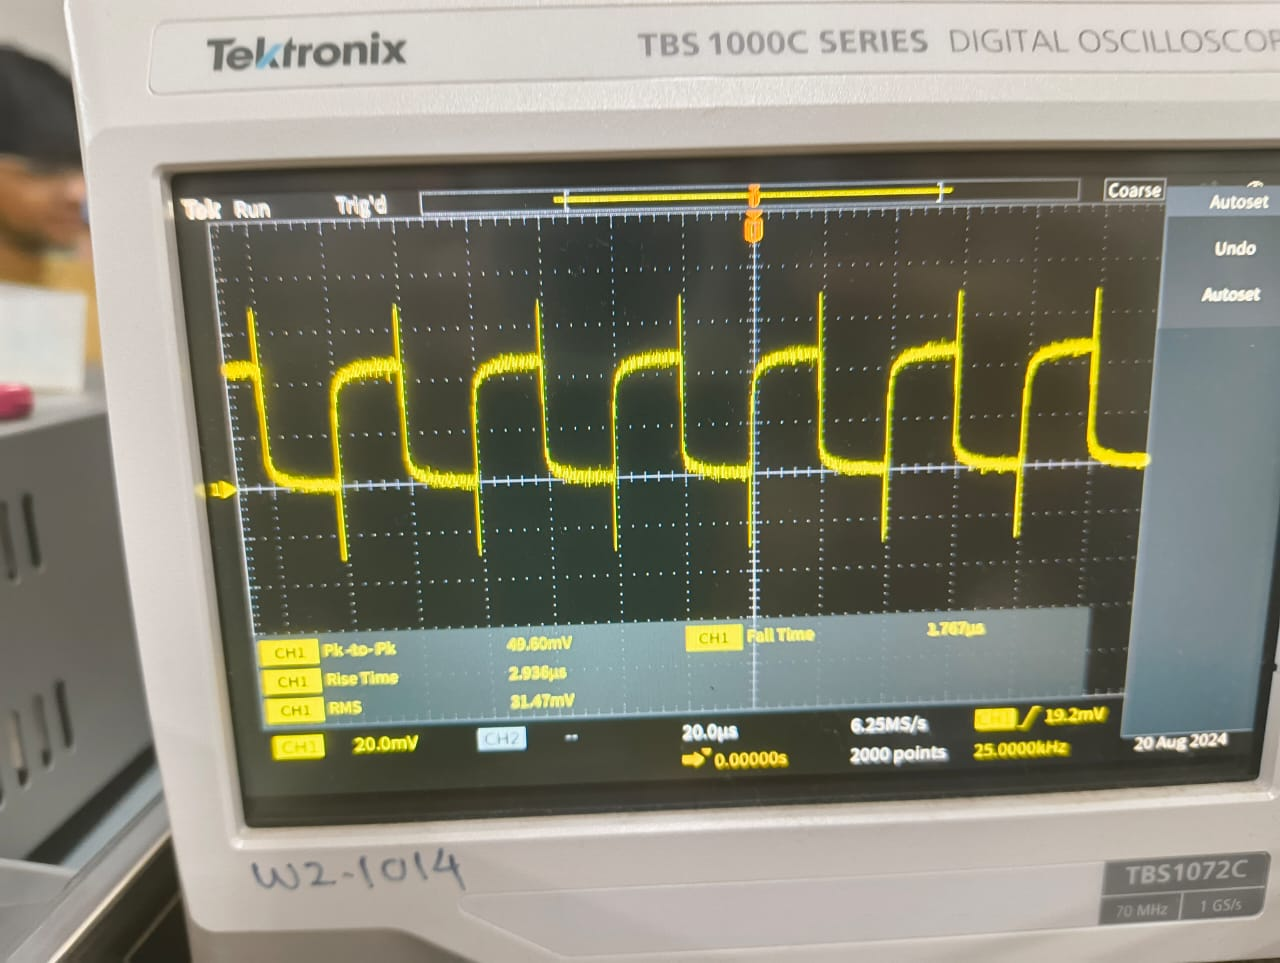
\includegraphics[width=0.8\linewidth]{25k.jpeg}
    \caption{For 25KHz}
\end{figure}

\begin{figure}[h!]
    \centering
    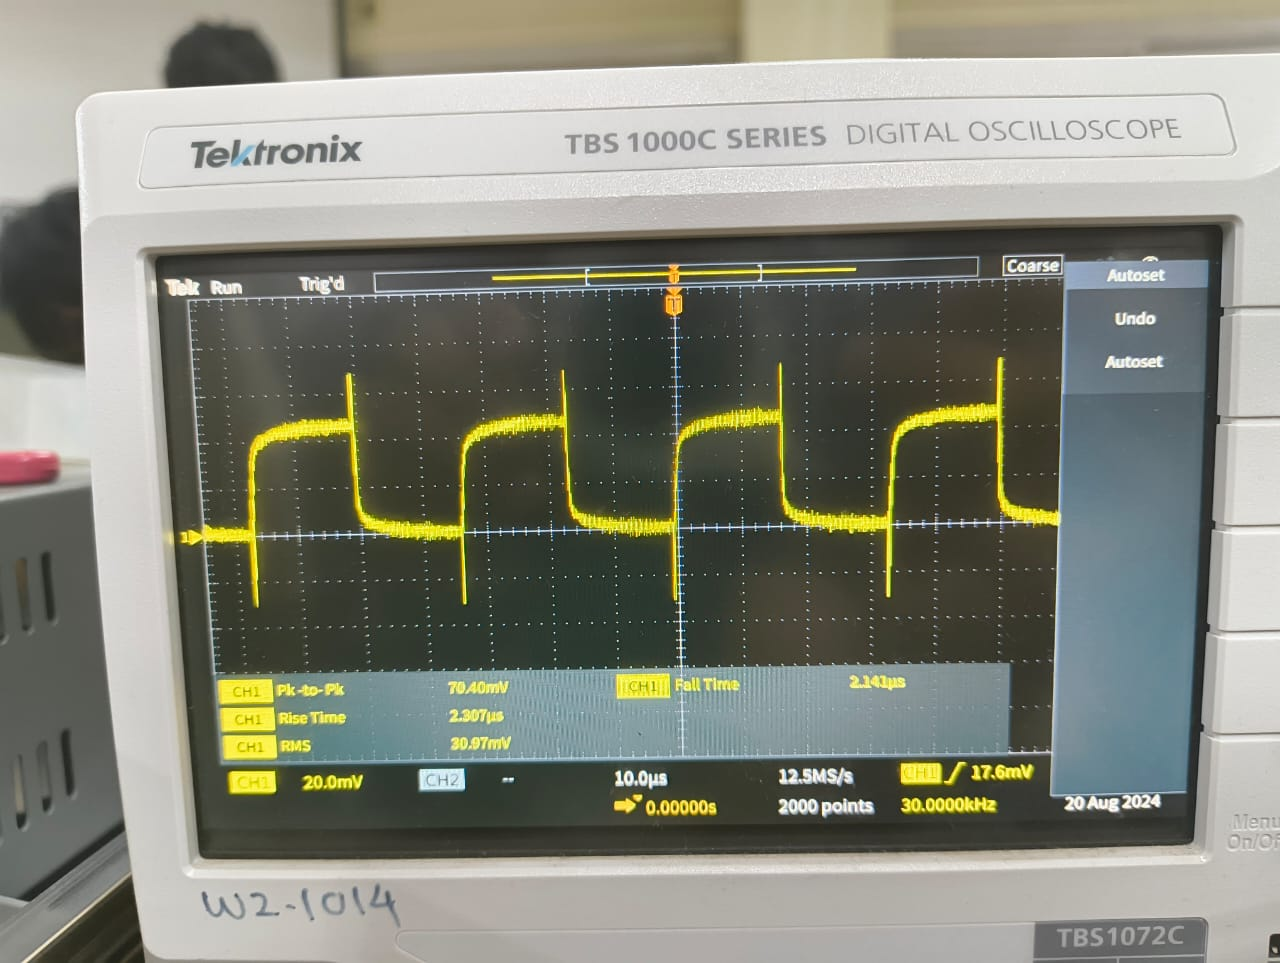
\includegraphics[width=0.8\linewidth]{30k.jpeg}
    \caption{For 30KHz}
\end{figure}

\begin{figure}[h!]
    \centering
    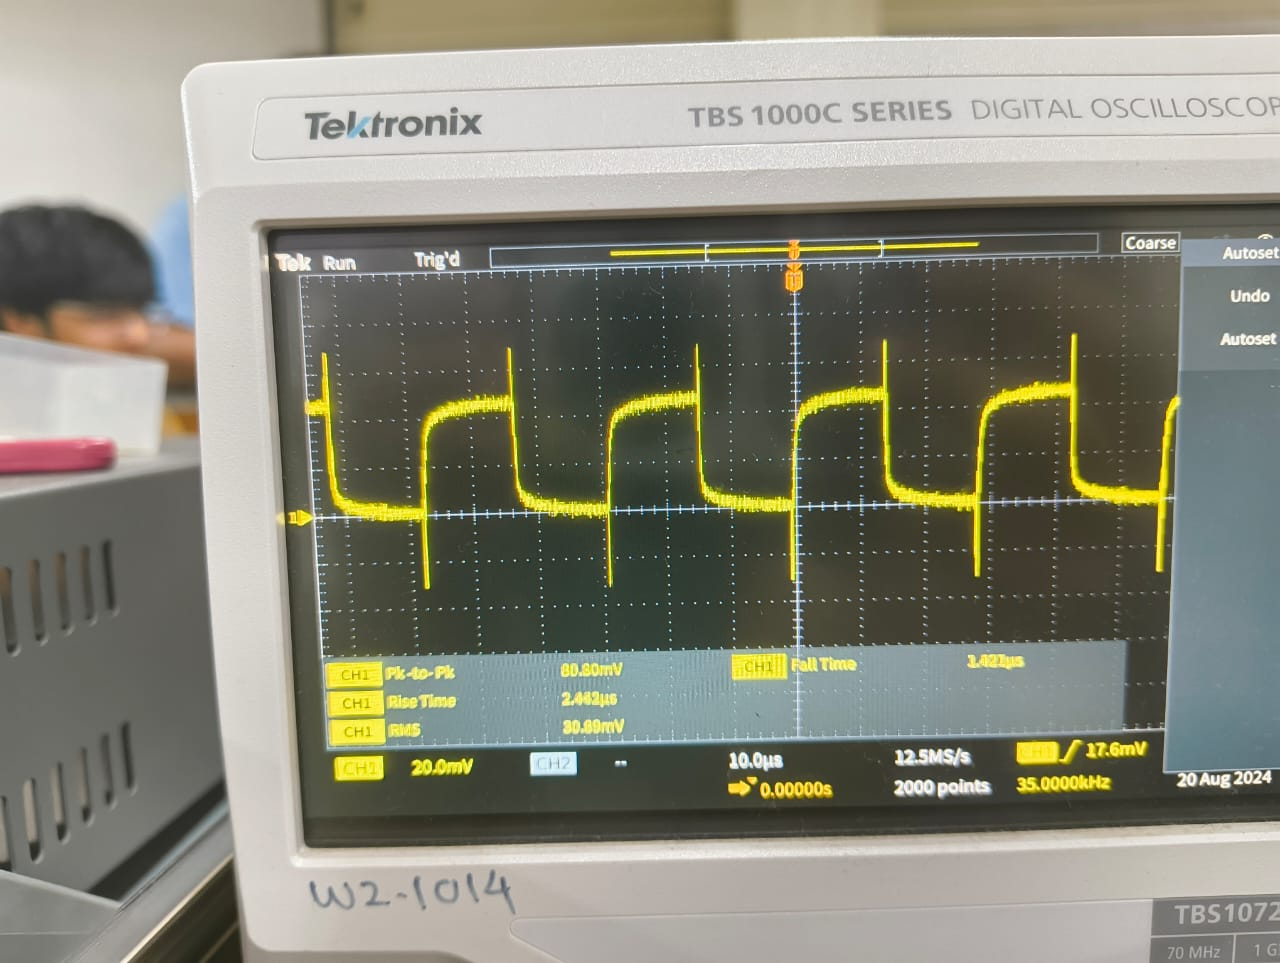
\includegraphics[width=0.8\linewidth]{35k.jpeg}
    \caption{For 35KHz}
\end{figure}

\end{document}
